\chapter{Background \label{ch:background}}
This chapter aims to give an introduction into the \acf{BEXUS} programme as a whole and the \acf{SETH} experiment as a part of this programme. Next the need for the \acf{ADS} is motivated and the measurement methods of the accelerometer and magnetometer explained.

\section{\acs{SETH} and the \acs{BEXUS} programme \label{sec:bg:seth_and_bx_programme}}

The first balloon of the \ac{BEXUS} programme, \textit{BEXUS 1}, launched on November 25$^{\mathrm{th}}$ 2002 at 15:53 UTC. Since then every year, except for 2003, 2020 and 2022, saw balloons being launched from the designated launch site \ac{ESRANGE} near the Swedish city of Kiruna \cite{IAC-08.E.1.1.4}\cite{bexus-campaign-history}.
The \acf{BX} programme is a bilateral programme between the \acf{DLR} and \acf{SNSA}. It offers university student teams the opportunity to build their own experiment and have it fly on a stratospheric balloon. The programme spans around one year and is constructed as a scaled-down version of a real space mission. The \acf{SETH} takes part in the 16th \ac{BEXUS} cycle and is expected to fly between the 3$^\mathrm{rd}$ of October 2025 and 13$^\mathrm{th}$ of October 2025 form \ac{ESRANGE}.

The purpose of \ac{SETH} is to investigate the angular dependency of particle radiation in the upper atmosphere. To this end a means of measuring the experiments attitude and heading while on the gondola is required.

The main source of radiation in the atmosphere are \acp{GCR} that hit the earth isotropically from all directions. In 1935 Erich Regener and Georg Pfotzer published an article in \textit{Nature} presenting a figure (see fig. \ref{fig:regener1935}) which shows the radiation intensity measured by three Geiger-Müller Counters stacked on top of each other to have an aperture angle of about 20$^\circ$ around the zenith \cite{regener-pfotzer-1935}.

\begin{figure}[H]
    \centering
    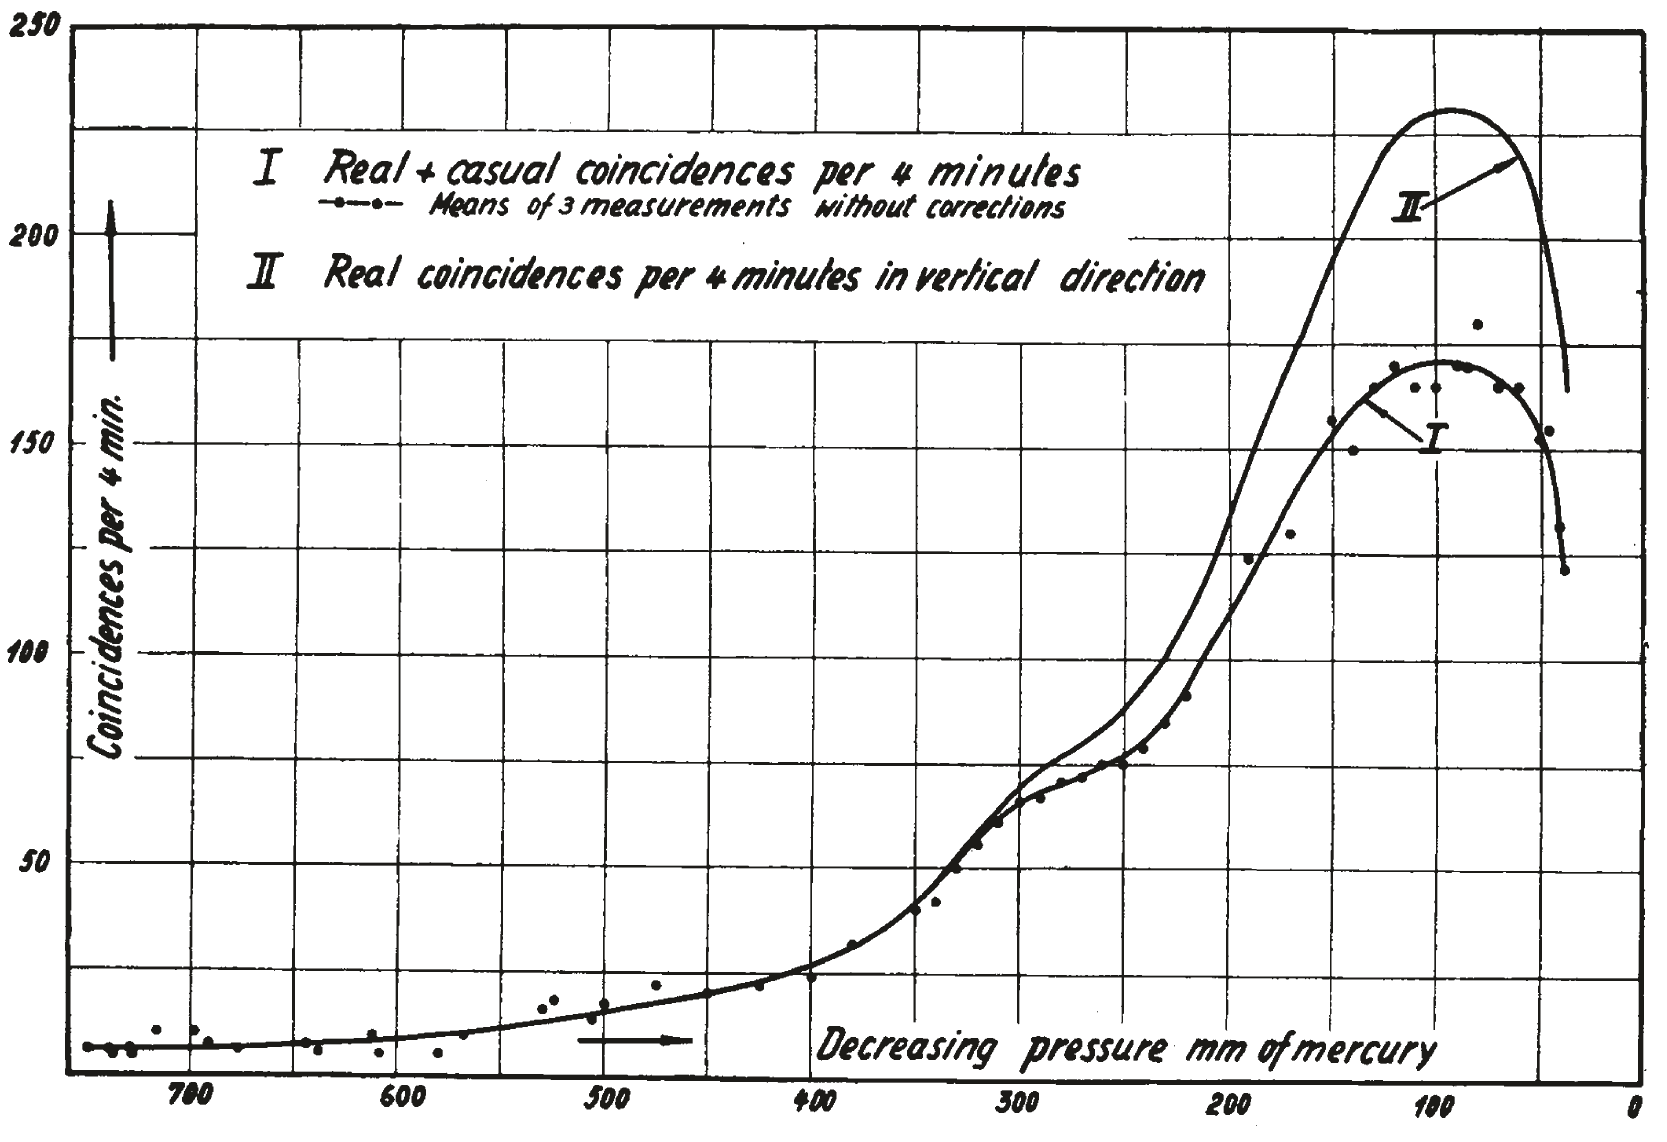
\includegraphics[width=0.8\linewidth]{images/01_background/original_regener_pfotzer.png}
    \caption[Regener-Pfotzer-Maximum as shown in \cite{regener-pfotzer-1935}]{Curve I shows the uncorrected coincidences per 4\,min. against ambient pressure in mm\ce{Hg}. Curve II shows the corrected coincidences taking the probability of coincidence counting against casual coincidences into account\cite{regener-pfotzer-1935}.}
    \label{fig:regener1935}
\end{figure}

Eighty Years later, the \ac{ADAM} \ac{BEXUS} Team around Dennis Trautwein showed that the fluence of particles for a given altitude varied with the zenith angle. Figure \ref{fig:martensen2015} taken from \cite{martensen2015} shows the angular distribution of particle fluence at an altitude of 27\,km.

\begin{figure}[H]
    \centering
    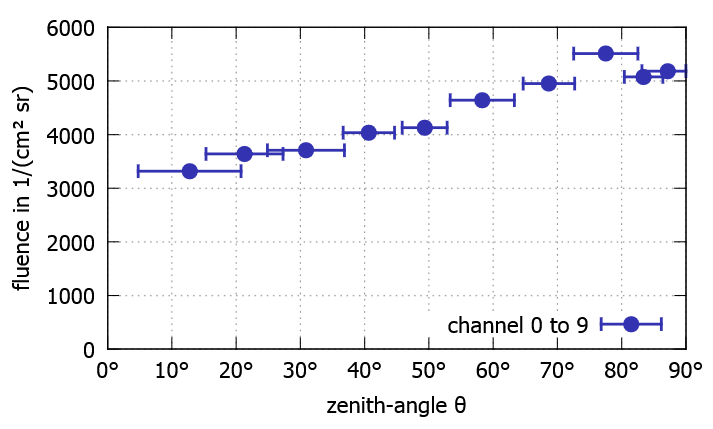
\includegraphics[width=0.6\linewidth]{images/01_background/martensen.png}
    \caption[Results of \acs{ADAM} at 27\,km]{Angular distribution of the charged particle fluence at an altitude of 27\,km \cite{martensen2015}.}
    \label{fig:martensen2015}
\end{figure}

Counting rate $C$ (coincidences per unit time) and isotropic Intensity $I_0$ (Fluence per unit time) share a linear relationship with the Geometrical Factor $G$ as coefficient, as is given in eq. \eqref{eq:sullivan}\cite{SULLIVAN19715}.
\begin{equation}
    C=G\cdot I_0
    \label{eq:sullivan}
\end{equation}

\newpage
The \ac{SETH} experiment has multiple well defined goals:

    \underline{\textbf{Primary Objectives}}
		\begin{description}\setlength\itemsep{-1em}
			\item[Obj. 1.1:] To measure Primary Galactic Cosmic Rays and secondary particles around the Regener-Pfotzer maximum and analyse its angular dependency. (Scientific)
			\item[Obj. 1.2:] To test a new electronics design featuring 48 signal channels . (Technical)
		\end{description}
	\underline{\textbf{Secondary Objectives}}
		\begin{description}\setlength\itemsep{-1em}
			\item[Obj. 2.1:] To measure the different particle species of Primary Galactic Cosmic Rays. (Scientific)
            \item[Obj. 2.2:] To measure showering of a very high energy electron in the \ac{BGO} detectors. (Scientific)
            \item[Obj. 2.3:] To measure the cardinal direction of the gondola. (Technical)
		\end{description}

The goals of \ac{SETH} which are the motivation for this thesis are Objectives 1.1 and 2.3: to measure the angular distribution of the Regener-Pfotzer-Maximum in the zenith and in the azimuthal angle and the determination of the gondolas cardinal direction (i.e. heading). A \ac{CAD} model of parts of the \ac{SETH} detector is shown in fig. \ref{fig:seth_cad}. The zenith and azimuthal angle of an incoming particle can be determined through the coincidence of two photodiodes (active area shown in orange).

\begin{figure}[H]
    \centering
    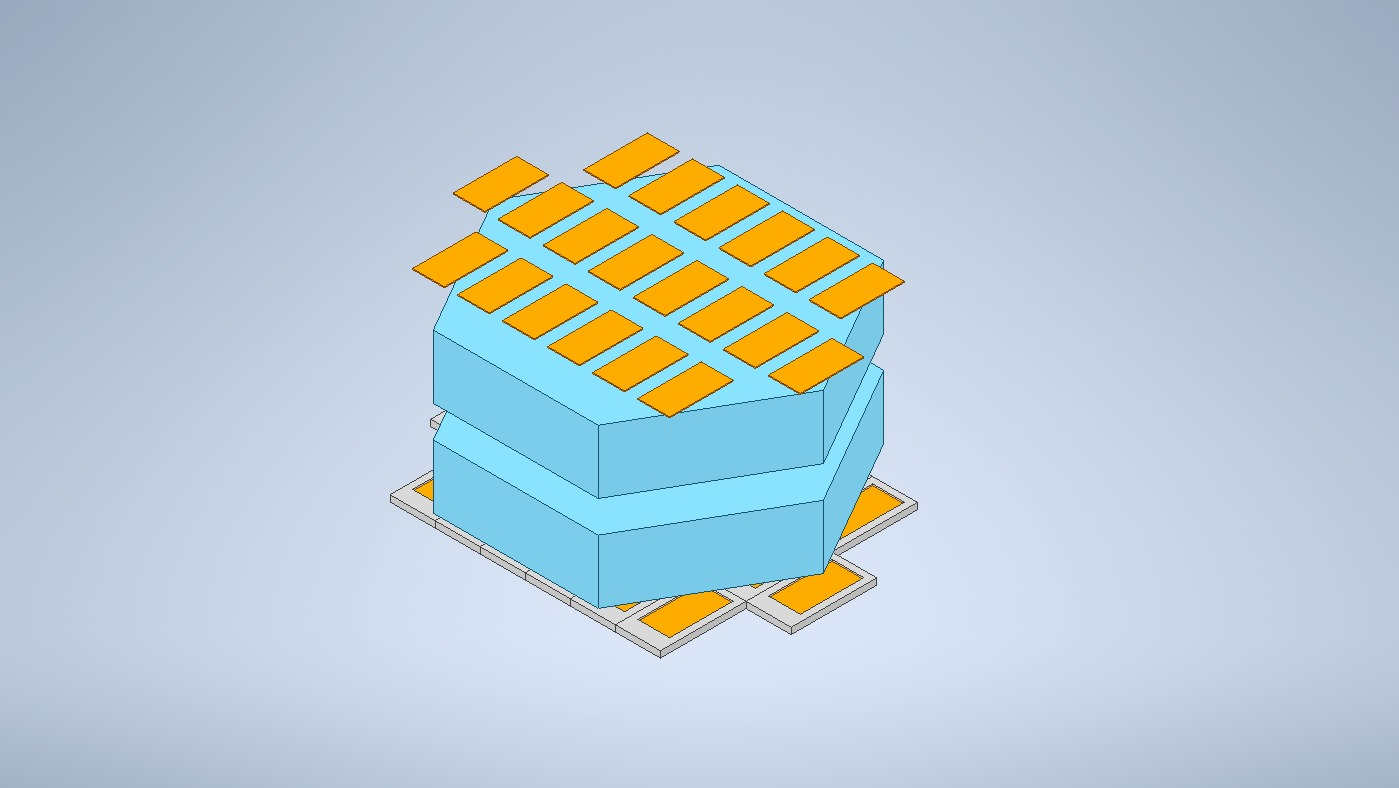
\includegraphics[width=0.5\linewidth, trim = {5cm 0cm 5cm 0cm}, clip]{images/01_background/SETH-Sketch.jpeg}
    \caption[\ac{SETH} detector sketch]{\ac{CAD} model of the \ac{SETH} detector showing the array of diodes.}
    \label{fig:seth_cad}
\end{figure}

The gondola hanging from the \ac{BEXUS} balloon does not have a fixed orientation in space. The wind will incite the gondola to rotate and swing during all phases of flight. Thus to get a reliable measurement of the angular distribution of the Regener-Pfotzer-Maximum in the azimuth domain, accurate heading information is required so as to know which direction particles travelling through the telescope hail from. The heading may occasionally be called yaw or azimuth.

\framebox[\linewidth][c]{\textbf{Objective 1.: The gondolas heading shall be measured.}}

As mentioned above, the gondola will also experience swinging or more accurately pitching and rolling. This is a deflection from the plane parallel to the local earths surface, split into the lateral and longitudinal axis of the gondola (for comparison see fig. \ref{fig:attitude}). As the gondola is a rigid body and all experiments are fixated, the attitude of the gondola as a whole is the same as the attitude of our experiment.

\framebox[\linewidth][c]{\textbf{Objective 2.: The gondolas attitude shall be measured.}}

\begin{figure}[H]
    \centering
    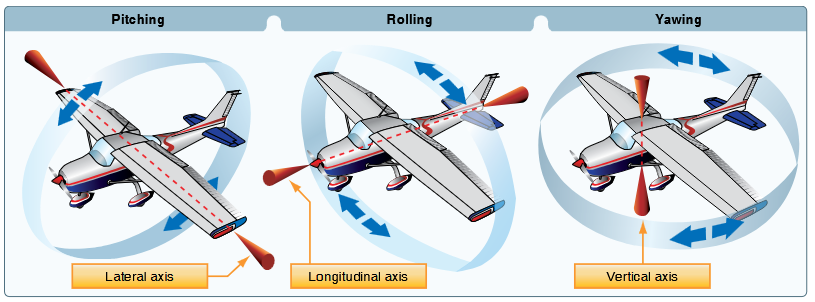
\includegraphics[width=0.5\linewidth]{images/01_background/axes_of_an_airplane.png}
    \caption[Axes of an airplane]{Axes of an airplane, from \cite{pilot-handbook}.}
    \label{fig:attitude}
\end{figure}

It is the job of the \ac{ADS} to fulfil objectives 1 and 2. This thesis will cover the implementation, calibration and preliminary testing of the \ac{ADS}.

\section{Magnetometers \label{sec:bg:magnetometers}}
To fulfil Objective 1, to determine the gondola's heading, a magnetometer is used. The 3-axis magnetometer will allow us to determine magnetic north and with the \ac{WMM} the local declination (i.e. the deviation from true north) can be calculated resulting in the gondolas heading. 

While many phenomena can be used to determine the magnitude and direction of a magnetic field, the sensor used for this thesis relies on tunnel magnetoresistance.

\section{Accelerometers \label{sec:bg:accelerometers}}
To fulfil objective 2

\section{Measurement Errors \label{sec:bg:measurement_errors}}
The sensing elements described in sections \ref{sec:bg:magnetometers} and \ref{sec:bg:accelerometers} each work in one dimension. To get a three-axis sensor, three sensing elements are assembled orthogonally to one another. In this automated process, errors in the alignment of the three sensing elements may occur. We will interpret the misalignment of the three sensing axes of a sensor as a $3\times3$ matrix $C_{m}$.

Due to mechanical stresses, unshielded magnetic fields, or other influences during production of the sensing elements they each may have a scale factor different from 1. This means when a field of magnitude 1 is applied the sensor may read 1.1, and 0.55 when a field of magnitude 0.5 is applied. In this case, the scale factor would be 1.1. As each sensing element may have experienced different conditions during production, we will consider one scale factor per axis, resulting in a $3\times1$ matrix $C_{sf}$.

The third error intrinsic to all 3-axis sensors is a zero bias, or null shift. This error may again have its origin during production of each sensing element and affects each axis differently. This error quantifies the offset, that the scaled measured value has from its true value. For example if no field is applied but the sensor reads a magnitude of 0.5 then that is the null shift. For the sensor as a whole, this is another $3\times1$ matrix $C_{zb}$.

While the errors introduced above are present in accelerometers and magnetometers alike the latter suffers from two more errors. These are soft iron and hard iron errors which are a natural part of the measurement of magnetic fields.\\
The hard iron errors $\delta\vec{B}$ are interfering magnetic fields from sources of constant magnetic fields around the sensor. Examples may be iron screws, nuts, or washers. This is a $3\times1$ matrix.

The last error to be discussed is a $3\times3$ soft iron error matrix $C_{si}$.

The measured quantities, denoted by the subscript "meas", can thus be expressed by the true vector fields as shown below. The superscripts $a$ and $b$ denote the accelerometer and magnetometer respectively.
\begin{align}
    \vec{G}_{meas}&=C^a_mC^a_{sf}\vec G+C_{zb}^a \\
    \vec{B}_{meas}&=C^b_mC^b_{sf}C^b_{si}(\vec{B}+\delta\vec{B})+C_{zb}^b
\end{align}